\subsection{Archivos de configuración}

Los archivos de configuración desempeñan un papel fundamental en el desarrollo y la operación de sistemas informáticos modernos al proporcionar una forma estructurada de definir variables y ajustes clave que modifican y parametrizan el comportamiento de los sistemas \autocite{van_der_hoek_configurable_1999}. Además, facilitan la modificación del sistema sin necesidad de acceder y modificar directamente el código fuente, lo que promueve la flexibilidad y la mantenibilidad.

Este epígrafe explora diversas técnicas y formatos utilizados para la configuración de aplicaciones, destacando su importancia en la gestión eficiente de la infraestructura y la personalización de comportamientos. Se analiza el uso de archivos de variables de entorno (.env) \autocite{pandey_guide_2022}, así como de JSON \autocite{erickson_what_2024,bray_javascript_2014} y YAML \autocite{ben-kiki_yaml_2021,redhat_what_2023} en combinación con JSON Schema \autocite{attouche_witness_2022,json_schema_json_2024} para la validación y estructuración de configuraciones. Aunque existen otros formatos como TOML [20], estos no tienen soporte para JSON Schema, lo cual carece de la capa adicional de seguridad y estructuración que es fundamental en muchos entornos de desarrollo. Este epígrafe proporciona una visión detallada de cómo estos archivos facilitan una configuración adaptable y robusta.

\textbf{JSON Schema}

JSON Schema o Esquema JSON es un estándar para la definición y validación de la estructura de documentos en distintos formatos. Proporciona un marco para especificar las propiedades requeridas, los tipos de datos, las restricciones de valores y otras reglas que los datos deben cumplir. JSON Schema no es un archivo de configuración por sí mismo, sino más bien una interfaz para asegurar que los archivos de configuración cumplan con las especificaciones esperadas \autocite{attouche_witness_2022,json_schema_json_2024}.

El uso de JSON Schema mejora la seguridad y la robustez de los sistemas al validar automáticamente la configuración antes de su aplicación, evitando errores y asegurando la conformidad con los requisitos del sistema \autocite{attouche_witness_2022,json_schema_json_2024}.

En la \autoref{fig:json-schema} se muestra un ejemplo de JSON Schema donde se definen 4 propiedades simples de disintos tipos y distintas restricciones. Por ejemplo prop1 se define como una cadena de caracteres, prop2 como un entero con valor máximo 100 y valor mínimo 0, prop3 un booleano, y prop4 como un arreglo que debe tener elementos únicos y un máximo de 3 elementos. A cada una de estas propiedades se les puede proveer de una descripción lo cual ayuda en la comprensión del propósito de la propiedad.

\begin{figure}[H]
    \centering
    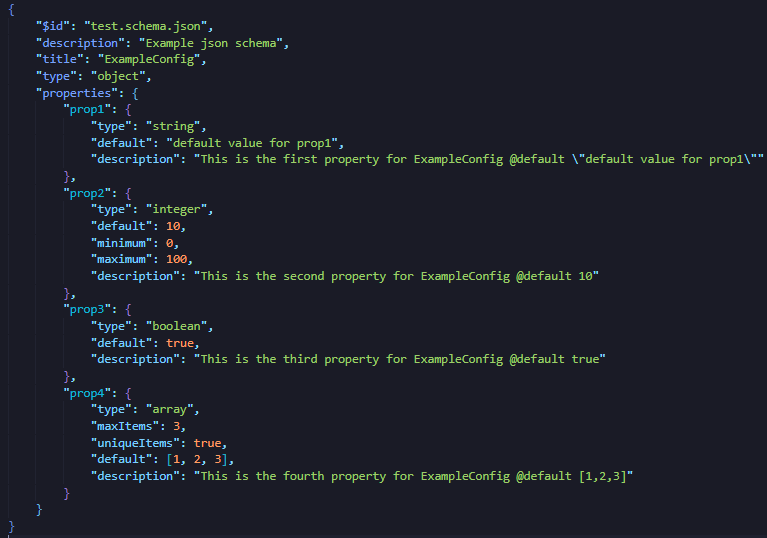
\includegraphics[width=\linewidth]{images/json-schema.png}
    \caption{Ejemplo de esquema JSON con varias propiedades de distintos tipos}
    \label{fig:json-schema}
\end{figure}

\textbf{JSON + JSON Schema}

Los archivos JSON son ampliamente utilizados para la configuración de aplicaciones debido a su simplicidad y compatibilidad con muchas herramientas y lenguajes de programación \autocite{erickson_what_2024}. Cuando se combinan con JSON Schema, estos archivos pueden ser validados para asegurar que cumplen con las especificaciones esperadas. Esto permite definir configuraciones de manera clara y estructurada, garantizando que los datos sean consistentes y conformes a los requisitos del sistema \autocite{bray_javascript_2014,attouche_witness_2022}.

En la \autoref{fig:json+jsonschema} se muestra un ejemplo de archivo JSON aplicando el esquema definido en la \autoref{fig:json-schema}. Se puede ver como establecer el esquema dota al archivo JSON de autocompletado en las propiedades, además de validaciones según las restricciones del esquema.

\begin{figure}[H]
    \centering
    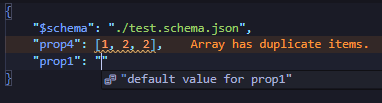
\includegraphics{images/json+jsonschema .png}
    \caption{Ejemplo de archivo JSON aplicando el esquema}
    \label{fig:json+jsonschema}
\end{figure}

\textbf{YAML + JSON Schema}

YAML es un formato de serialización de datos más legible que JSON (\autoref{fig:yaml-vs-json}) y ampliamente utilizado en la configuración de aplicaciones. Su sintaxis limpia y sencilla lo hace ideal para archivos de configuración \autocite{ben-kiki_yaml_2021,redhat_what_2023}. Al igual que JSON, los archivos YAML pueden ser validados utilizando JSON Schema, proporcionando una capa adicional de seguridad y estructuración. Esto combina la legibilidad de YAML con la robustez de la validación de JSON Schema, haciendo que las configuraciones sean tanto claras como seguras \autocite{attouche_witness_2022}.

En la \autoref{fig:yaml+jsonschema} se muestra un ejemplo de archivo YAML aplicando el esquema definido en la \autoref{fig:json-schema}. Se puede ver como establecer el esquema dota al archivo YAML de autocompletado en las propiedades, además de validaciones dependiendo de las restricciones del esquema.

\begin{figure}[H]
    \centering
    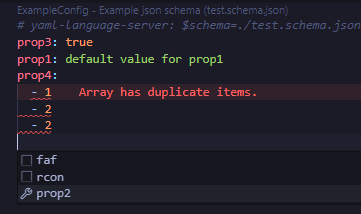
\includegraphics{images/yaml+jsonschema .png}
    \caption{Ejemplo de archivo YAML aplicando el esquema}
    \label{fig:yaml+jsonschema}
\end{figure}

\textbf{Variables de entorno (.env)}

Las variables de entorno son una técnica comúnmente utilizada para configurar aplicaciones. Estos archivos, generalmente con la extensión .env, permiten definir variables clave en un formato sencillo de clave-valor (\autoref{fig:env}), facilitando la gestión de configuraciones sensibles y específicas del entorno, como credenciales de acceso, URLs de servicios externos, y configuraciones de depuración \autocite{pandey_guide_2022}.

\begin{figure}[H]
    \centering
    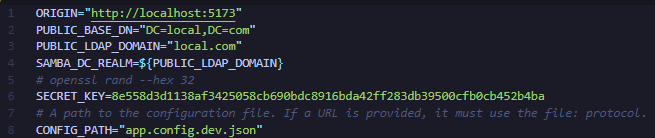
\includegraphics{images/env.png}
    \caption{Ejemplo de archivo .env}
    \label{fig:env}
\end{figure}

En la \autoref{table:config-files-comparison} se examinan aspectos como la facilidad de implementación, el soporte de tipos de datos, la capacidad de validación, la popularidad en diversos contextos de desarrollo, la complejidad de la sintaxis y el soporte nativo en el lenguaje Javascript. Esta información permitirá una comprensión detallada de cuándo y cómo utilizar cada formato para mejorar la configuración y la gestión de aplicaciones \autocite{pandey_guide_2022,aws_yaml_2023,eriksson_comparison_2011}.

\newgeometry{hmargin=0.5cm,vmargin=2cm}
\begin{longtable}{|p{3cm}|p{4.5cm}|p{5cm}|p{4.5cm}|}
    \caption{Comparación entre distintos estándares de archivos de configuración}
    \label{table:config-files-comparison}                                                                                                                                                                                                                                                                                                     \\
    \hline
    \textbf{Característica} & \textbf{.env}                                                        & \textbf{JSON + JSON schema}                                                                                                & \textbf{YAML + JSON schema}                                                                                 \\
    \hline
    \endfirsthead
    Facilidad de uso        & Alta: Requiere mínimo conocimiento técnico.                          & Media: Estructurado pero con una sintaxis muy estricta.                                                                    & Alta: Fácil de usar con herramientas y bibliotecas bien soportadas.                                         \\
    \hline
    Soporte de tipos        & Ninguno, todo son cadenas de texto                                   & Completo: Admite tipos como cadenas, números, booleanos, arrays, objetos, y más                                            & Completo: Soporta varios tipos de datos, incluidos mapas y listas.                                          \\
    \hline
    Validación de datos     & No: No tiene capacidad de validación                                 & Sí: Puede validar datos contra un esquema definido                                                                         & Sí: Es posible validar los datos contra un esquema predefinido                                              \\
    \hline
    Complejidad de sintaxis & Muy Baja: Sintaxis muy simple y directa                              & Media: Sintaxis detallada y estructurada                                                                                   & Baja: Sintaxis simple y directa                                                                             \\
    \hline
    Uso en aplicaciones     & Ideal para configuraciones sensibles al entorno y ambientes de CI/CD & Definición y validación de datos: Ideal para garantizar que los datos sean consistentes y conformes a las especificaciones & Configuración, automatización: Utilizado para definir configuraciones complejas y scripts de automatización \\
    \hline
    Popularidad             & Alta: Ampliamente utilizado en aplicaciones web y de software        & Alta: Ampliamente utilizado para validación de datos y definición de esquemas                                              & Alta: Popular en DevOps y administración de sistemas                                                        \\
    \hline
    Soporte nativo          & Sí                                                                   & Sí                                                                                                                         & No, se necesitan dependencias extra para parsearlo primero.                                                 \\
    \hline
\end{longtable}
\restoregeometry
